\documentclass[xcolor=x11names,compress]{beamer}

% -----------------------------------------------------------------------------------------
% The bit you should be interested in
%
% \usetheme[infolabcolours,num,forcecurve]{SmartSerif}
% \usetheme[bgcurve]{SmartSerif}
% \usetheme[num]{SmartSerif}
% \usetheme[bannerline=red]{SmartSerif}
% \usetheme[bannerbg=black]{SmartSerif}
% \usetheme[]{SmartSerif}
% 

\usetheme[]{SmartSerif}


% -----------------------------------------------------------------------------------------
% Other things for the sample
\usepackage{hyperref}

\usepackage{graphicx}
\graphicspath{ {./images/} }


% -----------------------------------------------------------------------------------------

\title{
    \includegraphics[scale=0.3]{logo_large.png}\\
    LWAC: Longitudinal Web as Corpus\vspace{15pt}}
\author{Stephen Wattam,\
Paul Rayson,\
Damon Berridge}
\institute[2013]{Lancaster University}
\date{\tiny \today}

\begin{document}

\maketitle

\section[Outline]{}
\frame{\tableofcontents}

% -----------------------------------------------------------------------------------------
%  About longitudinal sampling---why do it?
\section{Rationale}
\frame{\frametitle{About}
\begin{itemize}
    \item Monitor corpora are typically the go-to resosrce for temporal data
    \item Need for more formal sampling:
        \begin{itemize}
            \item Short-term effects online
            \item Changes to existing pages; content updates
            \item Technical aspects of WaC
        \end{itemize}
\end{itemize}    
}

\frame{\frametitle{Cohort Sampling}
\begin{itemize}
    \item Common longitudinal design
    \item Fits with open-source, URI-based corpus model
    \item Used elsewhere to disambiguate long- from short-term effects
        % BHPS, other national longitudinal studies
    \item Exposes technical and linguistic change over time
\end{itemize}    
}

\frame{\frametitle{Comparison}
\begin{itemize}
    \item Explain the confusing graph:
\end{itemize}    

\begin{center}
    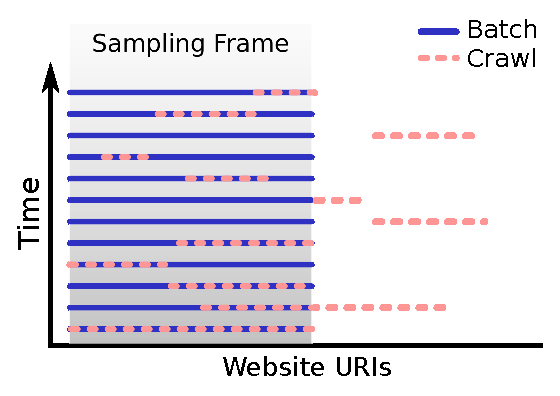
\includegraphics[scale=0.8]{samples.eps}
\end{center}


\note{\begin{itemize}
    \item Mention regularity of samples
    \item Mention the horizontal/vertical constraints being rigorous and reliable
\end{itemize}}
}



% -----------------------------------------------------------------------------------------
%  What longitudinal sampling is "all about", i.e. what properties it should have,
%  and the design principles for LWAC
\section{Design}

\frame{\frametitle{Sample Design 2}
\begin{itemize}
    \item Temporally homogenous samples
    \item Strict, regular sampling periods
    \item Vertical comparability
\end{itemize}    
}



\frame{\frametitle{Model}
\begin{itemize}
    \item A physical person accessing a web page using a typical home PC
    \item Support for ``realistic'' redirects, encoding handling, headers, protocols
    \item Measurement of network and content data
    \item 
    \item 
\end{itemize}    
}


\frame{\frametitle{Reliability}
\begin{itemize}
    \item No `skew' on sampling intervals
    \item Data security across crashes/restarts (atomicity)
    \item Error reporting
    \item Stability for long-term runs
    \item 
\end{itemize}    
}

\frame{\frametitle{Scalability}
\begin{itemize}
    \item Must scale over link count and time
    \item Platform limitations:
    \begin{itemize}
        \item All tools $< O(N)$ memory, $\leq O(N)$ time and disk space
        \item Specific disk format limits (inodes)
        \item Kernel limits (open io handles)
    \end{itemize}
\end{itemize}    

% During testing I left LWAC running a benchmark over the weekend, 
% and returned to find it had filled my hard disk with 3.8 million copies (479GB) of the same
% html file

}



% -----------------------------------------------------------------------------------------
%  About the form LWAC takes
\section{Implementation}

\frame{\frametitle{Overview}
\begin{itemize}
    \item UNIX-model tool set (cross-platform?)
    \item Written in Ruby using cURL
    \item Distributed client-cerver design
\end{itemize}    

\begin{center}
    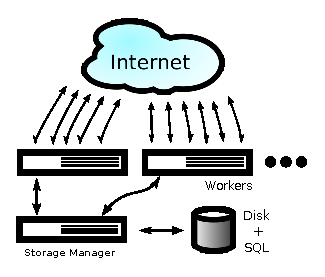
\includegraphics[scale=0.8]{arch.eps}
\end{center}


\note{\begin{itemize}
    \item 
\end{itemize}}

}


\frame{\frametitle{Tools}
\begin{itemize}
    \item \textbf{Import}---Imports links into the database
    \item \textbf{Server}---Controls sampling policy and data storage
    \item \textbf{Client}---Makes requests to the web, normalises data
    \item \textbf{Export}---Extracts metadata and text from the server's corpus directory
\end{itemize}    



\note{\begin{itemize}
    \item Go through these, p'raps?
\end{itemize}}

}





\frame{\frametitle{Server}
\begin{itemize}
    \item Manages link cohort
    \item Ensures atomic data access
    \item Controls sampling policy centrally
    \item Logs everything in obscene detail
\end{itemize}
}

\frame{\frametitle{Client}
\begin{itemize}
    \item Highly parallel downloads (using cURL)
    \item Able to normalise character set, respond to redirects
    \item Persistent, configured by server on-the-fly (set and forget)
    \item Able to run on low powered machines
\end{itemize}    
}

\frame{\frametitle{Import/Export}
\begin{itemize}
    \item Import arbitrary URL lists (supports duplicates)
    \item Export to CSV, XML or arbitrary templates
    \item Export using filters and data normalisation
\end{itemize}    
}




\subsection{Client Imitation}
\frame{\frametitle{Stealth Features}
\begin{itemize}
    \item Clients send configurable request headers
        % UA, referrer, accept-encoding
    \item Redirects may be set to typical browser limits
    \item Timeouts can be set to mimic user behaviour
    \item 
\end{itemize}    
}


\subsection{Data Storage}
\frame{\frametitle{Data Storage}
\begin{itemize}
    \item MySQL or SQLite3 for links
    \item Versioned `NoSQL' for data
    \item Configurable serialisation format
    \item Accessible by Server, Sample or Data-level features
    \item $\approx 120$ variables stored on each request
\end{itemize}    
}


\subsection{Performance}
\frame{\frametitle{Performance}
% TODO
\begin{itemize}
    \item TODO, dig out old notebook.
\end{itemize}    
}

\subsection{Resource Usage}
\frame{\frametitle{Resource Use}
\begin{itemize}
    \item Memory usage $O(1)$ for client and server
    \item Memory usage defined by batch size:
        \begin{itemize}
            \item Server: $(\textit{clients} \times \textit{batch\_size} \times \textit{link\_size}) + (\textit{batch\_size} \times \textit{max\_resource\_size})$
            \item Client: $\textit{in\_progress} \times \textit{max\_resource\_size}$ (using disk cache)
        \end{itemize}
    \item Disk usage $O(N)$ for server, $O(1)$ for client.

    \item Practically around 120-200MB for the application, 1-200MB for data.
\end{itemize}

\note{\begin{itemize}
    \item Practically server is about 200MB, with ruby and dep libraries in RAM
    \item The client is usually a bit less, around 120MB, but can grow if configured to do so.
    \item Payload sizes: server: client+about 10MB, client: usually up to 200MB or so
\end{itemize}}

}


% -----------------------------------------------------------------------------------------
%  A rough overview of use
%  possibly a demo?
\section{Use}

\frame{\frametitle{Basic Workflow}
  \begin{columns}
    \begin{column}{.7\linewidth}
        \begin{enumerate}
            \item Find links of interest ([Web]BootCaT)
            \item Import links (\texttt{lwac import})
            \item Set up clients (\texttt{lwac client})
            \item Run server (\texttt{lwac server})
            \item Drink coffee (RFC 2324)
            \item Export data (\texttt{lwac export})
            \item Do science
        \end{enumerate}    
    \end{column}
    \begin{column}{.25\linewidth}
        \includegraphics[scale=0.1]{coffee.jpg}
    \end{column}
  \end{columns}



\note{\begin{itemize}
    \item Step through workflow
    \item You may wish to use a process monitor on the client and server
    \item You can export before the server is done (and even delete old samples from the disk)
    \item RFC2324 is HTCPCP: the Hyper Text Coffee Pot Control Protocol
\end{itemize}}
}


\frame{\frametitle{Use Cases}
\begin{itemize}
    \item 
    \item 
    \item 
    \item 
    \item 
\end{itemize}    
}



\frame{\frametitle{Etiquette}
\begin{itemize}
    \item LWAC is capable of DDOS-style throughput
    \item Normally lists of links contain references to each server a few times
        %(their frequency is usually proportional to the popularity of the website, which means bigger sites can handle the traffic anyway)
    \item Within-sample rate controlled by the parallel connection limit
    \item Between-sample rate defined by sample period
\end{itemize}    


\note{\begin{itemize}
    \item Not NETiquette.  God I hate that term.
    \item Parallelism is a more helpful way to limit hits to servers
    \item It's a bad idea for the quality of data to slow down each sample
    \item Nothing can be done about between-sample time, it's defined by your experimental design
\end{itemize}}

}


% -----------------------------------------------------------------------------------------
%  Summary/Marketing plug
\section{Summary}
\frame{\frametitle{Summary}
\begin{itemize}
    \item LWAC makes longitudinal sampling easy (ish!)
    \item Will sample over long- or short-term
    \item Modest resource requirements
    \item Insane throughput
    \item Absurdly configurable
    \item Fully documented
\end{itemize} 


\note{\begin{itemize}
    \item 
\end{itemize}}
}


\frame{\frametitle{The Last Slide}

    \begin{center}

    \url{http://ucrel.lancs.ac.uk/LWAC/}\\
    \vspace{25pt}
    TODO: when demo if demo\\
    \vspace{25pt}
    Suggestions/comments/bug reports welcome!\\
    \texttt{s.wattam@lancaster.ac.uk}

\end{center}

\note{\begin{itemize}
    \item 
\end{itemize}}
}

% -----------------------------------------------------------------------------------------
%  Auxiliary slides

% \frame{\frametitle{About}
% \begin{itemize}
%     \item 
% \end{itemize}    
% }

% -----------------------------------------------------------------------------------------
\end{document}
